\section{Diskussion}
\label{sec:Diskussion}
Allgemein fällt auf, dass die Fehler der Messwerte, die sich aus der Standardabweichung ergeben, wesentlich größer
als die angegebenen baubedingten Fehler sind. Da der Versuchsaufbau korrekt umgesetzt wurde, bleibt als Fehlerquelle
lediglich die Genauigkeit der Bauelemente. Dabei ist fest zu stellen, dass die Bauelemente alle relativ alt sind und
empfindlich auf Stöße reagieren, da die Anschlussbuchsen locker sind und deshalb die Anschlüsse nicht richtig
funktionieren.\\
Weiterhin ist die Abweichung für $L_{16}$ und $R_{16}$ ziemlich groß, obwohl mit die Werte einmal mit einer 
Induktivitäts- und einmal mit einer Maxwellbrücke bestimmt wurden. Die Werte von $L_{16}$ weichen um $641,13\,\%$
voneinander ab. Die Werte von $R_{16}$ weichen um $177,41\,\%$ voneinader ab.\\


\section{Messwerte}
\label{sec:Messwerte}

\begin{figure}
  \centering
  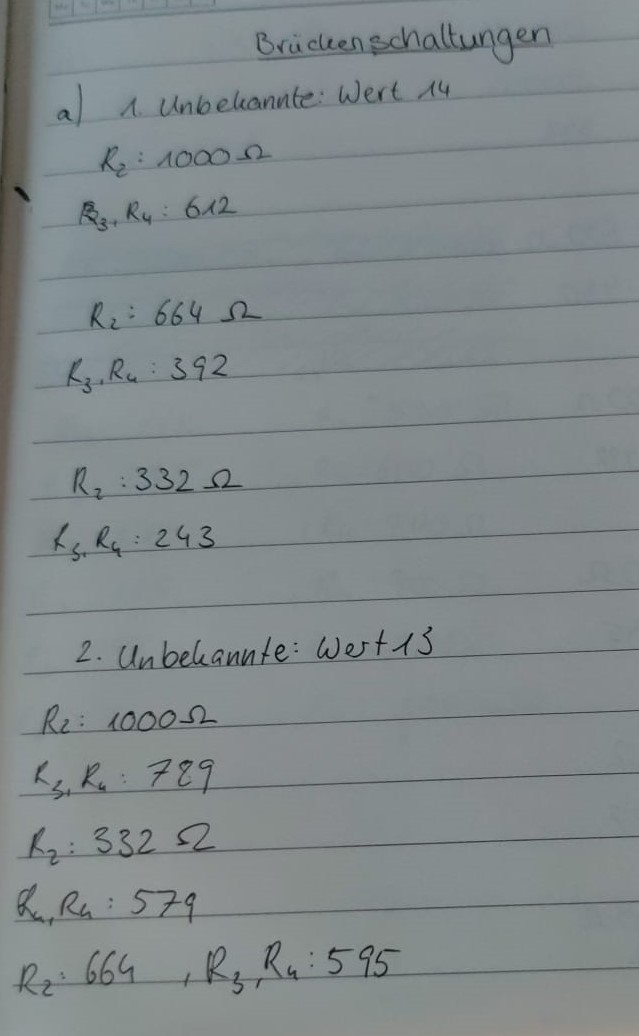
\includegraphics[width=0.7\textwidth]{M_a).jpeg}
  \caption{Messdaten 1}
  \label{fig:M1}
\end{figure}

\begin{figure}
  \centering
  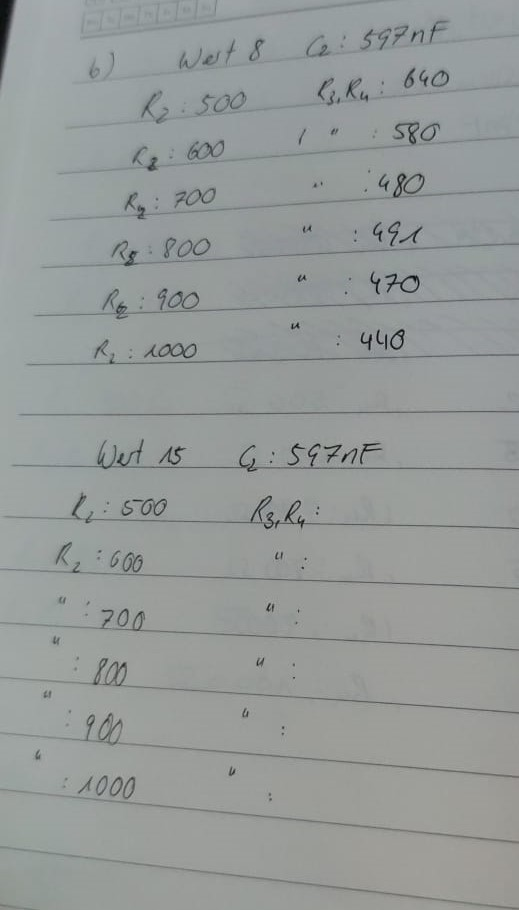
\includegraphics[width=0.7\textwidth]{M_b).jpeg}
  \caption{Messdaten 2}
  \label{fig:M2}
\end{figure}

\begin{figure}
  \centering
  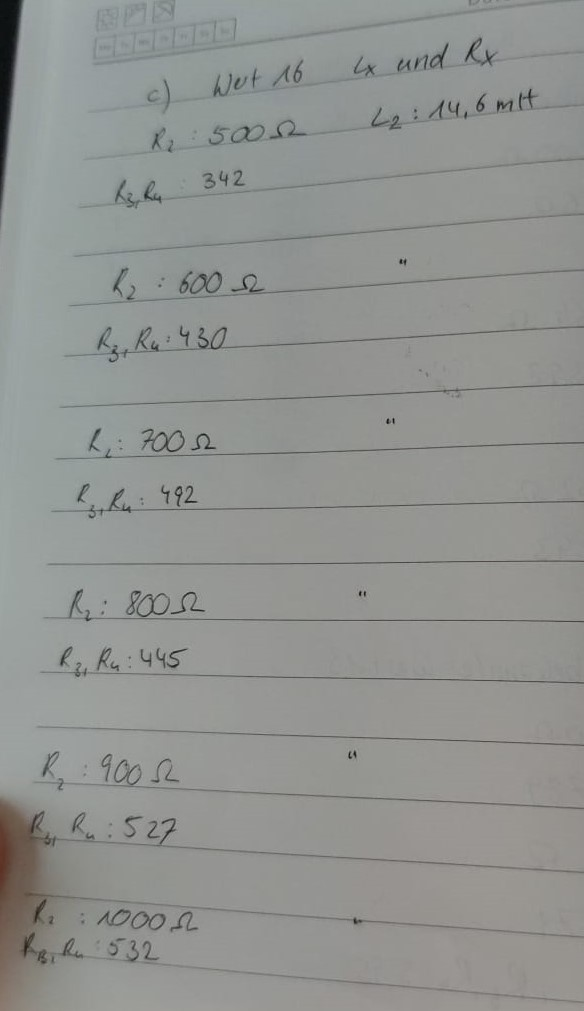
\includegraphics[width=0.7\textwidth]{M_c).jpeg}
  \caption{Messdaten 3}
  \label{fig:M3}
\end{figure}

\begin{figure}
  \centering
  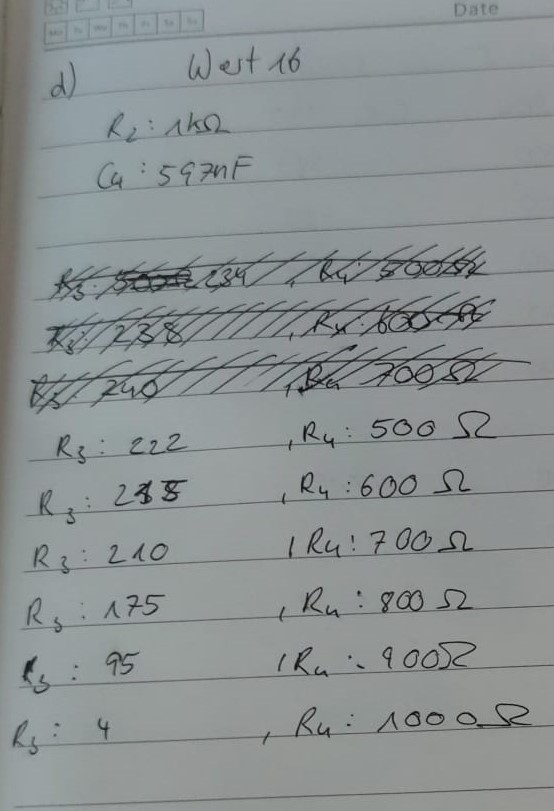
\includegraphics[width=0.7\textwidth]{M_d).jpeg}
  \caption{Messdaten 4}
  \label{fig:M4}
\end{figure}

\begin{figure}
  \centering
  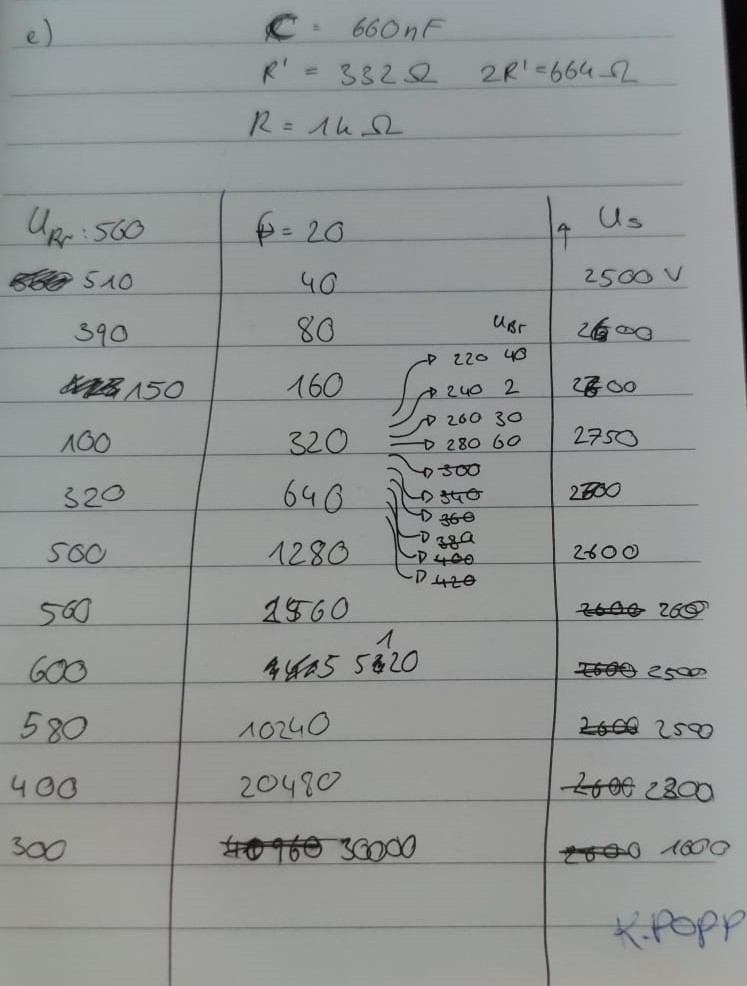
\includegraphics[width=0.7\textwidth]{M_e).jpeg}
  \caption{Messdaten 5}
  \label{fig:M5}
\end{figure}
  